\section{Experimental Design}

In this section we lay the foundations and discuss the design decisions of our system. 
First we present the details of our user study and data collection. 
We then introduce the design concepts behind \sys{}, our automated pipeline for clustering users into debloating sets and assigning each set to a differently-debloated web application.
Figure~\ref{fig:environment_preparation} shows the high level steps including the data collection and clustering, followed by the preparation of the content delivery environment to serve debloated web applications.

\subsection{User Study - Identifying common web application features from the perspective of experienced administrators}

To understand how experienced users interact with web applications, we conduct the following user study. 
We hire our user-study participants by advertising paid projects on popular freelancing platforms, such as, Upwork~\cite{upwork}. 
After reviewing the resumes and interviewing the candidates, we hire experienced freelancers with 2-10 years of expertise on web development and system administration. 
We specifically interviewed candidates who mentioned phpMyAdmin, WordPress, or Magento on their resume. We focused on these web applications since they were used in the ``Less is More'' study of Amin Azad et al.~\cite{lessismore}, allowing us to compare and contrast our findings with theirs. 

The main goal of this user study is to understand which features in the web applications in our dataset are commonly used among developers and administrators, and which features are relatively unpopular, used by only a fraction of administrators.

\subsubsection{User Study Tasks}

\begin{figure}[t]
    \centering
    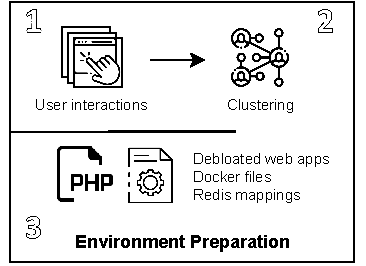
\includegraphics[]{figures/dbltr/EnvironmentPreparation.pdf}
    \caption{During the training phase, we collect user interaction code coverage traces to generate clusters. Based on these clusters, specialized debloated copies of web applications are produced for each cluster.}
    \label{fig:environment_preparation}
\end{figure}

\begin{figure*}[h]
    \centering
    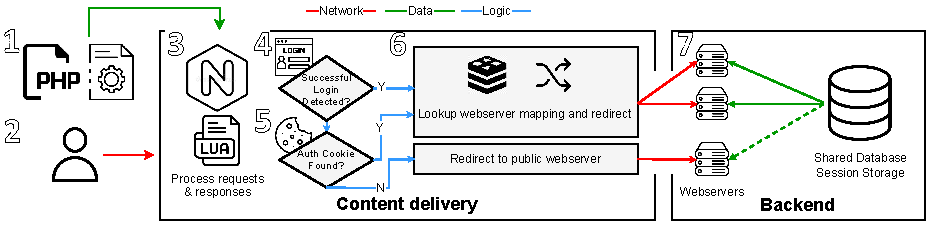
\includegraphics[]{figures/dbltr/RoleModelsFlow.pdf}
    \caption{System Architecture of \sys{}. In Step 1, we provide the debloated web applications and user to cluster mappings to \sys{}'s content delivery module. User requests (2) are processed by \sys{}'s reverse-proxy (Step 3). After identifying the identity of the user (Steps 4-6), \sys{} internally routes the requests to the custom debloated web applications (Step 7).}
	\label{fig:system_architecture}
\end{figure*}

The task description for each project consists of an overview of the user study, the background required to participate, and the expected deliverables. 
Moreover, we included the information about the consent to participate in our study and described the information that we collect (i.e., server-side logs and code-coverage information). 

After interviewing the participants and reviewing their resumes, we hired 20 experts for each web application for a total of 60 experts on phpMyAdmin, WordPress, and Magento. 
We compensate the participants at the rate of \$15 per hour.

During the pilot experiments for the user study, we realized that not every freelancer is familiar with the concept of a user study. 
More importantly, to avoid future disputes, freelancers preferred to work on a predefined list of tasks and deliverables. 

Based on these observations, we defined two milestones for our user study. 
First, we asked our participants to provide a list of web application features that they commonly use in their daily tasks and projects. 
Most of our participants listed both maintenance and administration tasks. 
Among the common tasks, we observed verification of the functionality of the website (e.g., registering as new customers, submitting orders, etc.), maintenance tasks (e.g., backups, import data, etc.) and even search-engine optimization. 

For the second milestone, we asked our participants to spend 1 hour of their time on our instrumented web applications and perform the tasks that they listed earlier. 
This process provided them with the list of deliverables and expectations, and also enabled us to validate their effort on this project. 

For freelancing platforms that provide a time-tracking utility, we use this feature to verify the participation of users together with cross-validating their task report with our code-coverage traces. 
For submissions that did not follow our guidelines (e.g., did not spend enough time, skipped the majority of tasks in the reports, etc.) we would ask the participants to revise their submission. 

\textbf{IRB Approval} Since our experiments involved the assistance of real users, we obtained an Institutional Review Board (IRB) approval for our user study. 
Upon providing thorough details of our tasks and the human interactions, along with the information that we collect from the users, we obtained IRB approval on May 27, 2020. 

\subsubsection{Setup of Web Applications}

To facilitate the setup of web applications for our user study participants, we prepared the following environments:

\begin{itemize}
    \item \textbf{phpMyAdmin:} We provide phpMyAdmin version 5.1.0, with multiple pre-populated databases including a WordPress, and a Magento database.
    \item \textbf{WordPress:} Our setup consists of the version 5.8 of WordPress with an admin account, over 20 blog posts, multiple pages pages, and comments. 
    \item \textbf{Magento:} We setup Magento 2.3.5 and configured the ``Sample data'' package that includes an inventory of over 1,000 products. 
\end{itemize}

Each participant received their own instance with the admin credentials on a unique subdomain. 
We re-create the same environment as ``Less is More'' to collect the usage traces from user interactions in the form of file and line coverage information. 

Through out this user study, we interviewed over 110 individuals, some of whom decided not to participate in our study due to reasons such as non-recurring and short-term nature of our tasks, their busy schedule, etc.
Overall, we spent numerous weeks interviewing our participants and following up with them to ensure the timely delivery of their tasks. The cost of this experiment was approximately \$1,000, most of which was used to pay the administrators in our user study and the remainder to pay for domain names and the hosting of virtual machines on public clouds.

\subsection{Debloating Pipeline}

In this section we describe \sys{}, a dynamic debloating pipeline. 
\sys{} is able to identify web-application users with similar usage profiles (i.e., roles), and create debloated applications that are tailored to the needs of users in each profile. 


Unlike previous one-size-fits-all approaches, application users with specific usage patterns do not need to inherit the whole code-base from other users with vastly different usage behaviors. 
A concrete example of this effect becomes apparent in the usage traces of WordPress. 
Certain administrators focus on the content, and the SEO. 
Therefore, they mostly interact with blog posts and page content, meta tags, and keywords. 
Conversely, another distinct group of administrators focused on changing the appearance of the website by installing new themes, and plugins such as ``Elementor'' that provides an easy interface to modify the appearance of the website. 
In this scenario, by providing the ability to install new plugins to the first group, we are unnecessarily increasing their privileges beyond what they really require. 

For certain web applications, their role-based, access-control mechanisms can limit, to a certain extent, unnecessary capabilities.
Unfortunately many PHP applications that provide administrative features lack this ability (e.g., phpMyAdmin). 
Moreover, the provided roles do not always match the real-world requirements of users. For instance, WordPress comes with only 6 hardcoded roles ranging from Super Admin to Subscriber. 
The benefit of our approach is that we dynamically identify the required web application features based on runtime traces. 

This effect is most significant when applications do not provide fine-grained permission management. 
For instance, using the classic ``single debloated application for all users'' approach, a super admin would share the codebase with data-entry users or even unauthenticated public users. 

Moreover, by clustering users with similar feature usage in the same group, we decrease the likelihood of breaking web application functionality due to removal of code if another user in the same cluster exercised the desired functionality. 
This is in contrast to user-specific debloating where each individual receives their own copy of the target web application based on their exclusive usage patterns. 
We provide a quantitative analysis of this effect in Section~\ref{sec:augmented_coverage}.

\subsubsection{Producing the debloated web applications}

\sys{} extracts the list of exercised files from usage traces. 
PHP file paths and names are effective indicators of the underlying feature corresponding to each file. 
Most commonly, web application source files are partitioned under directories that indicate the feature they implement. 
Moreover, for external dependencies (i.e., composer packages), the file-path includes the name of the module that the files belong to. 

Based on this information, we cluster file paths using the K-means clustering algorithm, into 2 to \emph{N} clusters, with \emph{N} denoting the total number of web application users (in this case, 20).  

\sys{} then produces the following artifacts:
\begin{itemize}
    \item \( \frac{N \times (N - 1)}{2} \) debloated variants of web applications.
    \item Configuration files for the reverse-proxy and the web servers to host the debloated web applications.
    \item Information about the mapping of users to debloating clusters.
\end{itemize}

\subsubsection{Routing users to debloating clusters}

One of the design requirements of \sys{} is seamless user experience. 
Therefore, we incorporate a reverse-proxy that identifies user login information and routes any post-authentication traffic to specialized containers which include debloated variants of the main application customized for the user. 

\sys{}'s reverse-proxy takes a config file for each web application. 
This file informs the proxy of how to identify successful login request-response pairs, the form field that contains the username and the session cookie name to track the user past authentication. 

This information is stored along with the user to web application mappings in an in-memory datastore. 
For authenticated users, the proxy extracts the session cookie, queries the datastore for the web server id for the user and routes the traffic to the appropriate debloated web application. 
From the user's perspective, there is no observable effect while this routing is taking place. Due to the architecture of \sys{}, two users can both be visiting the same URL at the same time, yet accessing radically different (i.e., debloated to match their needs) web applications under the hood. 

\subsubsection{Sharing web application state between web server instances}

Each debloated web application instance is produced from the same source code. 
Nevertheless, the state of each web application depends on the database, cookies, and the session storage. 

In order to keep the state of all web applications synchronized, we connect all of them to the same database instance in the docker environment. 
Moreover, directories that include the session information are mounted as a single volume across all web application instances. 
By sharing this volume, users that authenticate on one copy of the application and are redirected to another debloated instance will maintain their authenticated session cookie. This separation of the session store from web servers is a mainstream principle of scalable web applications allowing requests from the same user to be served by multiple web-server instances~\cite{scalability-book}.
Finally, since web browsers are responsible for maintaining the valid cookies, after routing users to different debloated web application instances served over the same URL, the cookies are automatically transferred along with future requests. 
